\documentclass[a4paper,12pt]{report}
\usepackage{hyperref}
\usepackage{graphicx}
\usepackage{multicol}
\usepackage{color}
\usepackage{caption}
\usepackage{setspace}
\usepackage{amssymb,amsmath}     
\usepackage{tikz}
\usepackage{float}
\usepackage{csquotes}
\usetikzlibrary{decorations.pathreplacing}
%\usepackage{amsfonts,amsrefs}
\usepackage{bm}          
\usepackage{tabularx}
\usepackage{enumerate}
%\usepackage[authoryear,square,sort]{natbib}
%\usepackage[linesnumbered,ruled,vlined]{algorithm2e}
\usepackage{algorithmic}
\usepackage{lscape}
\makeatletter
\def\verbatim@font{\linespread{1}\normalfont\ttfamily}
\makeatother
\usepackage{pgfpages}

\begin{document}
%titlepage
\thispagestyle{empty}
\begin{center}
    \centering
%Thesis title
    {\uppercase{\Large \textbf{Wave Scattering by Submerged Elastic Vertical Barriers}\par}}
    \vspace{3cm}
    
    % Otago logo
    
\includegraphics[width=4cm]{logo.pdf}
    \vspace{2cm}
    
%Author's name
    {\Large {\bf Xavier Nuttall}\par}
    \vspace{2cm}
    
%Degree
    {\large A dissertation submitted in partial fulfilment of the requirements of the degree of Bachelor of Science with Honours\par}
    \vspace{1cm}
    
% Institution
    {\large Department of Mathematics and Statistics\\University of Otago
%Te Tari P\={a}ngarau me te Tatauranga, Te Whare W\={a}nanga o Ot\={a}go
\par}
    \vspace{1cm}
    
%Date
    {\large {Month, Year}}

\end{center}


\setcounter{secnumdepth}{-2}% 

\tableofcontents

\setcounter{secnumdepth}{4}% 

\chapter{Introduction}
In recent years, there has been a growing interest in coastal protection strategies due to increased coastal erosion stemming from climate change and rising sea levels. A significant factor contributing to coastal erosion is the presence of \enquote{ocean gravity waves} with periods between 5-25s, which will be referred to as \enquote{waves} throughout, as in \cite{MosigJohannesErnstManfred2018Cwim}. One widely adopted method for coastal protection is the use of wave attenuation systems~\cite{cite...}, designed to dissipate the energy of waves before they reach the coastline. One mechanism of attenuation is scattering, which reflects and traps wave energy, thereby protecting coastal areas~\cite{Wilks_Montiel_Wakes_2022}. Modelling the scattering caused by these attenuation systems is crucial for understanding their effectiveness in reducing wave energy and protecting coastal regions.

A significant body of research has been devoted to modelling wave scattering by surface-piercing barriers~\cite{10.1093/imamat/35.3.339, PARSONS1994129, Porter1995ComplementaryAT}, submerged vertical barriers~\cite{Porter1995ComplementaryAT}, surface-piercing elastic barriers~\cite{doi:10.1137/090756557}, horizontal floating elastic structures~\cite{WU1995301, MontielFabienFranck2012NaEA}, and submerged porous vertical barriers~\cite{VIJAY2020102206}. However, there is little research into scattering by submerged elastic vertical barriers~\cite{elasticVerticalBerrier2013}. One frequently used approach when solving these scattering problems is the \enquote{eigenfunction matching method} also known as the \enquote{eigenfunction expansion-matching method} \cite{WU1995301, 10.1029/2007JC004434, 10.1093/imamat/35.3.339}. However, this method can be computationally expensive and may not be suited for problems with sharp singularities, such as those involving vertical barriers as shown in \cite{jmse13030398}. Another common approach are the galerkin methods, as used by \cite{Porter1995ComplementaryAT,10.1093/imamat/35.3.339,PARSONS1994129} in problems of rigid structures. This method was shown to be computationally more efficient than the eigenfunction matching method, for problems with sharp singularities like in those we are considering \cite{jmse13030398}. This approach is also commonly used in problems of flexible/elastic beams \cite{Lian2024}, a potentially similar problem to the one we are considering. 


This work aims to build upon the existing literature on submerged elastic vertical barriers, with a focus on ground-standing barriers. To start with, we will consider the problem of rigid plates.



\chapter{Rigid Vertical Barrier}
\section{Mathematical Model}
\label{sec:mathModel}
We consider the scattering of linear water waves by a submerged, bottom-standing vertical barrier located at $x=0$ in a two-dimensional Cartesian coordinate system. Here, $x$ denotes the horizontal direction of wave propagation (positive to the right), and $z$ is the vertical direction, positive upwards. The undisturbed free surface is at $z=0$, and the flat seabed is at $z=-h$. The vertical barrier extends from the seabed at $z=-h$ up to its tip at $z=-d$, so occupise space between $-h < z < -d$.

To apply classical linear water-wave theory, we assume the wave amplitude $\eta(x,t)$ is small compared to both the wavelength and the water depth, allowing the free surface to be approximated by $z=0$. The fluid is taken to be inviscid, incompressible, and initially at irrotational, so the flow remains irrotational. The waves are assumed to be time-harmonic with angular frequency $\omega$. We impose a no-flow boundary condition at the seabed and a no-flow condition at the barrier. The velocity potential $\Phi(x,z,t)$, under the time-harmonic assumption, can be written as:

\begin{equation}
\label{eq:time-harmonic}
\Phi(x,z,t) = \text{Re}(\phi(x,z)\exp(-i\omega t)).
\end{equation}
The spacial velocity potential $\phi(x,z)$ satisfies the boundary value problem (BVP):
\begin{align}
\label{eq:irrotational}
\nabla^2 \phi = 0,&  &&(x,z) \text{ not in the barrier}, \\
\label{eq:noFlowGround}
\partial_z \phi = 0,&  &&z = -h, \\
\label{eq:freeSurface}
\partial_z \phi = -\frac{\omega^2}{g}\phi,&  &&z = 0, \\
\label{eq:noFlowBarrier}
\partial_x \phi= 0,&  &&x = 0, -d < z < -h.
\end{align}

\begin{figure}[h]
\centering
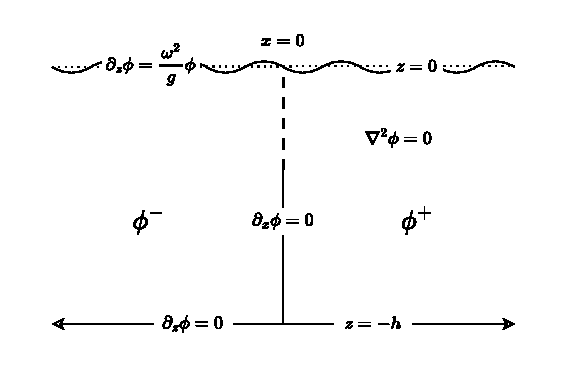
\includegraphics[width=12cm]{bvp-figure.pdf}
\caption{Diagram of the BVP}
\label{fig:bvp}
\end{figure}


The free surface condition (\ref{eq:freeSurface}) is the linearized kinematic boundary condition, derived from the non-stationary Bernoulli equation under the assumption of time-harmonic motion, with $g$ denoting the acceleration due to gravity~\cite{alma9938079562602711}. We partition the domain into two subdomains: $L = \{(x, z) \in \mathbb{R}^2 \mid x \leq 0\}$ (to the left of the barrier) and $R = \{(x, z) \in \mathbb{R}^2 \mid x \geq 0\}$ (to the right of the barrier). The governing equations (\ref{eq:irrotational}--\ref{eq:noFlowBarrier}) apply within each subdomain, while at the interface above the barrier ($x=0$, $-d < z < 0$), we enforce continuity of both the velocity potential and its $x$-derivative (velocity):
\begin{align}
\label{eq:phiEquality}
\phi^- = \phi^+, &&  x=0, -d < z < -h,\\
\label{eq:phiPartialEquality}
\partial_x\phi^- = \partial_x\phi^+, &&  x=0, -d < z < -h.
\end{align}
By applying separation of variables, the general solution to the governing equations (\ref{eq:irrotational}--\ref{eq:noFlowBarrier}) can be expressed as:
\begin{equation}
\label{eq:phiGeneralDefinition}
\phi(x,z) = \sum_{n=0}^{\infty} \big(\alpha_n\exp(ik_nx) + \beta_n\exp(-ik_nx)\big)\psi_n(z).
\end{equation}
Here, $\alpha_n$ and $\beta_n$ are the amplitudes of the left and right-oriented modes respectively, $i = \sqrt{-1}$, and
\begin{equation}
\label{eq:psiDefinition}
    \psi_n(z) = \cosh(k_n(z+h)),
\end{equation}
are the vertical orthogonal eigenfunctions. The wavenumbers $k_n$ in (\ref{eq:psiDefinition}) and (\ref{eq:phiGeneralDefinition}) are the (real and complex) roots of the linear dispersion relation:
\begin{equation}
\label{eq:waveNumbers}
\omega^2 = gk_n \tanh(k_n h),
\end{equation}
where $g$ is the acceleration due to gravity and $h$ is the total water depth.

Let $\phi^-(x,z)$ and $\phi^+(x,z)$ denote the velocity potentials in the $L$ and $R$ subdomains, respectively. The general solution in each subdomain can be expressed as:
\begin{align}
\label{eq:phiMinusDefinition}
\phi^-(x,z) &= \sum_{n=0}^{\infty} \left(A_n \exp(ik_n x) + B_n\exp(-ik_n x)\right)\psi_n(z),\\
\label{eq:phiPlusDefinition}
\phi^+(x,z) &= \sum_{n=0}^{\infty} \left(C_n\exp(ik_n x)+ D_n\exp(-ik_n x)\right)\psi_n(z),
\end{align}
where $A_0$ and $D_0$ correspond to the amplitudes of the left and right incident waves, respectively, and $B_n$ and $C_n$ are the coefficients for the reflected and transmitted modes. For the case of a single incident wave propagating from the left, we set $A_0 = 1$, $A_n = 0$ for $n \geq 1$, and $D_n = 0$ for all $n$. 

To enforce continuity of the horizontal velocity across the interface above the barrier ($x=0$, $-d < z < 0$), we introduce an auxiliary function $u(z)$ defined by
\begin{equation}
\label{eq:auxDefinition}
u(z) = \partial_x \phi^-(0,z) = \partial_x \phi^+(0,z).
\end{equation}
This function encapsulates the jump in the horizontal velocity at the interface between the two subdomains.
\section{Collocation}
The collocation method serves as a straightforward baseline against which more advanced or efficient methods can be compared. In this approach, we select a set of $M+1$ evenly spaced collocation points $\{z_k\}_{k=0}^{M}$ within the interval $[-h, 0]$, where $z_k = -h + k\frac{h}{M}$ for $k = 0, 1, \ldots, M$. At each collocation point, we enforce that the residual between the left and right subdomain solutions vanishes. For numerical computation, we truncate the infinite series in equations~\eqref{eq:phiMinusDefinition} and~\eqref{eq:phiPlusDefinition} to $N$ terms.
Then applying \ref{eq:phiMinusDefinition} and \ref{eq:phiPlusDefinition} into the above (\ref{eq:auxDefinition}) we have:
\begin{align}
\label{eq:auxMinusEquality}
u(z) &= \sum_{n=0}^{N} \big(A_nik_n - B_nik_n\big)\psi_n(z),\\
\label{eq:auxPlusEquality}
&= \sum_{n=0}^{N} \big(C_nik_n - D_nik_n\big)\psi_n(z).
\end{align}
Now  we multiply \eqref{eq:auxMinusEquality} by $\psi_m(z)$ and integrate with respect to $z$ over the interval $[-h, 0]$. By the orthogonality of the eigenfunctions $\psi_n(z)$, $\int_{-h}^0 \psi_m(\xi)\psi_n(\xi) d\xi = 0$ for $m \neq n$, this yields:
\begin{align}
\label{eq:auxMinusIntegrate}
U_m &= \int_{-h}^{0}\sum_{n=0}^{N} \big(A_nik_n - B_nik_n\big)\psi_n(\xi)\psi_m(\xi)d\xi,\nonumber\\
&= \sum_{n=0}^{N} \big(A_nik_n - B_nik_n\big)\int_{-h}^{0}\psi_n(\xi)\psi_m(\xi)d\xi,\nonumber\\
&= (A_m - B_m)P_mik_m
\end{align}
Where $U_m = \int^0_{-h}u(\xi) \psi_m(\xi) d\xi$ and $P_m = \int^0_{-h}\phi_m^2(\xi) d\xi$. Following the same process for \ref{eq:auxPlusEquality} we have:
\begin{align}
\label{eq:auxPlusIntegrate}
U_m &= (C_m - D_m)P_mik_m
\end{align}
Using \ref{eq:auxMinusIntegrate}, \ref{eq:auxPlusIntegrate}, \ref{eq:phiEquality}, \ref{eq:noFlowBarrier}, \ref{eq:auxDefinition} and $A_{n>0} = D_n = 0$, we obtain:
\begin{equation}
\label{eq:colocationSystem}
\psi_0(z) = \int_{-d}^0 K(z,\xi) u(\xi) d\xi.
\end{equation}
Here, the kernel is given by
\[
K(z,\xi) = \sum_{m=0}^{N} \frac{\psi_m(z)\psi_m(\xi)}{P_m i k_m}.
\]
We now discretize the integral equation~\eqref{eq:colocationSystem} by a numerical quadrature rule such as the trapezoidal rule at the collocation points $\{z_k\}$. This yields a linear system for the unknown values $u(z_k)$. Once these auxiliary values are computed, we can approximate $U_m$ and subsequently use equations~\eqref{eq:auxMinusIntegrate} and~\eqref{eq:auxPlusIntegrate} to solve for the coefficients $B_n$ and $C_n$.
\subsection{Convergence Analysis}


\section{Galerkin Method}
In this method, we approximate the solution $u(z)$ as a truncated sum of basis functions. We want these basis functions to encapsulate the singular behaviour at the tip of the barrier, caused by the change in velocity ($\partial_x \phi$) as you approach the tip from the \ref{eq:noFlowBarrier} condition. [explain the singularity as square root]. So we approximate $u(z)$ with truncation $W$ as,
\begin{equation}
\label{eq:galerkinApprox}
u(z) \approx \sum_{i=0}^{W} c_i v_i(z),
\end{equation}
where $c_i$ are the coefficients to be determined and,\\ $\displaystyle v_i(z) = ((h-d)^2-(h+z)^2)^{-1/2}T_{2i}\Big(\frac{z+h}{h-d}\Big)$, where $T_i$ are Chebyshev polynomials of the first kind. Then using this approximation in \ref{eq:colocationSystem} we have,
\begin{equation}
\label{eq:galerkinSystem}
\psi_0(z) = \int_{-d}^0 K(z,\xi) \sum_{i=0}^{W} c_i v_i(\xi) d\xi.
\end{equation}

Multiplying both sides by $v_m(z)$ and integrating over $z$ from $-d$ to $0$,
\begin{align}
\label{eq:galerkinIntegrate}
V_{0,m} &= \int_{-d}^0 \int_{-d}^0 K(z,\xi) \sum_{j=0}^{W} c_j v_j(\xi)  d\xi v_m(z) dz\nonumber\\
&= \sum_{j=0}^{W} c_j \int_{-d}^0 \int_{-d}^0 K(z,\xi) v_j(\xi)  d\xi v_m(z) dz\nonumber\\
&= \sum_{j=0}^{W} c_j \int_{-d}^0 \int_{-d}^0 \sum^N_{n=0} (ik_n P_n)^{-1} \phi_n(z)\phi_n(\xi) v_j(\xi) d\xi v_m(z) dz\nonumber\\
&= \sum_{j=0}^{W} c_j \sum^N_{n=0} (ik_n P_n)^{-1} \int_{-d}^0  \phi_n(\xi) v_j(\xi) d\xi \int_{-d}^0\phi_n(z) v_m(z) dz \nonumber\\
&= \sum_{j=0}^{W} c_j \sum^N_{n=0} (ik_n P_n)^{-1}  V_{n,j} V_{n,m}.
\end{align}
Where $V_{k,j} = \int_{-d}^0 \phi_k(z) v_j(z) dz$. We can then solve this system of equations for the coefficients $c_j$. Follwoing this we obtain an approximation of $u(z)$ to solve for the coefficients $B_n$ and $C_n$ in \ref{eq:auxMinusIntegrate} and \ref{eq:auxPlusIntegrate}, using the approximation,
\begin{equation}
\label{eq:galerkinApproxU}
U_m = \int_{-h}^{0} u(\xi) \psi_m(\xi) d\xi \approx \sum_{j=0}^{W} c_j V_{m,j},
\end{equation}
and the closed form solution \cite{bateman1954} to the $V_{m,j}$ integrals,
\begin{equation}
\label{eq:VIntegral}
V_{m,j} = \int_{-d}^{0} \phi_m(z) v_j(z) dz = (-1)^j \frac{\pi}{2} J_{2j}(ik_m(h-d)).
\end{equation}
         
%\clearpage
\addcontentsline{toc}{chapter}{Bibliography}
\bibliographystyle{amsplain}
\bibliography{HonsRefs}

\newpage
\appendix


\end{document}
